\documentclass[tikz,border=8pt]{standalone}
\usepackage{amsmath}
\usepackage{pgfplots}
\pgfplotsset{compat=1.18}
\usetikzlibrary{arrows.meta,decorations.pathmorphing}
\definecolor{ink}{HTML}{21352F}
\definecolor{teal}{HTML}{087F7B}
\definecolor{gold}{HTML}{C58B2A}
\definecolor{blue}{HTML}{4B77A8}
\definecolor{rose}{HTML}{B65A62}
\begin{document}
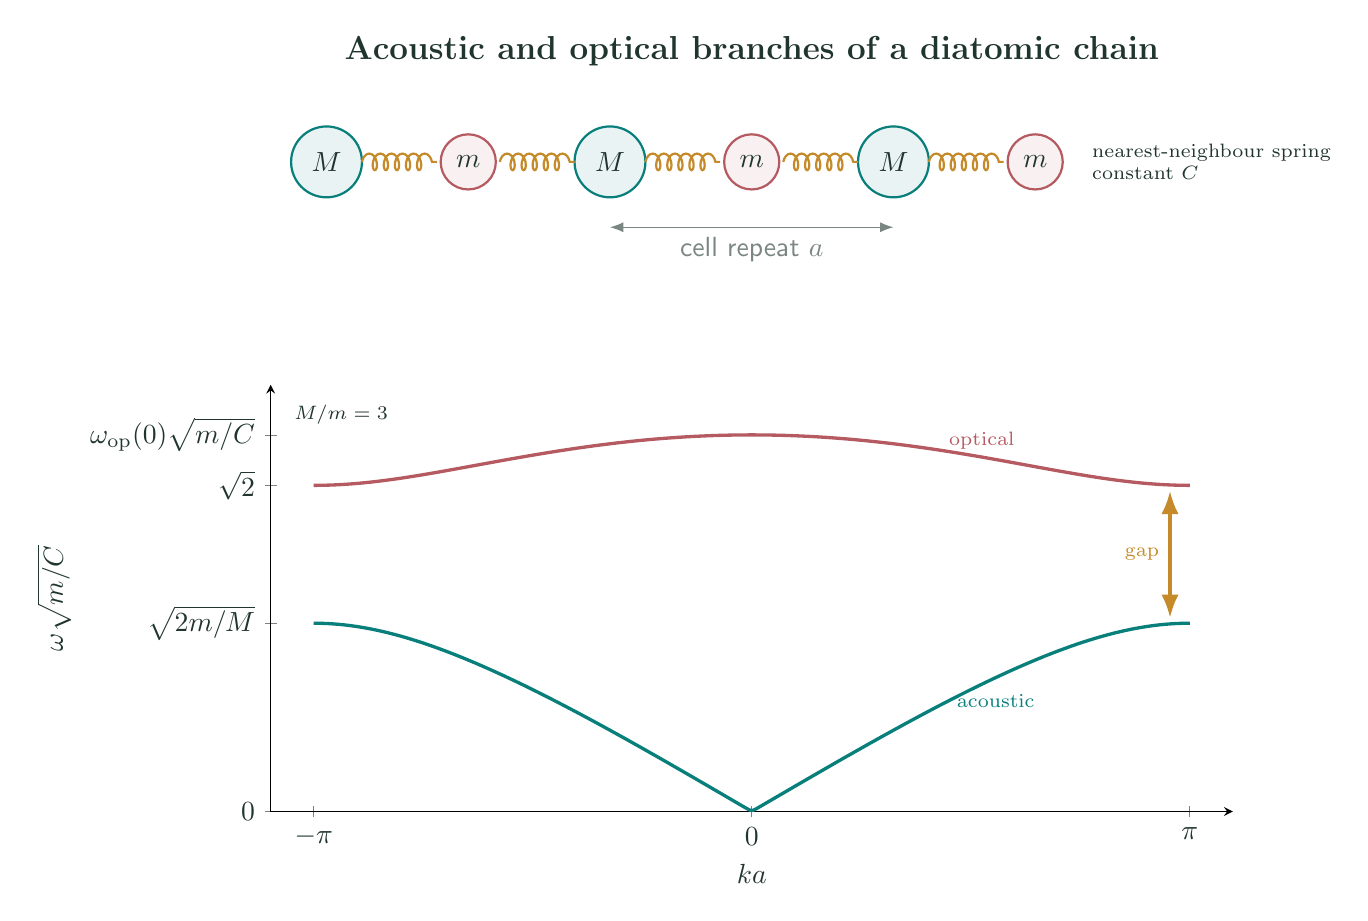
\begin{tikzpicture}[font=\sffamily,text=ink,>=Latex]
  \node[font=\bfseries\large] at (0,4.15) {Acoustic and optical branches of a diatomic chain};
  \foreach \x in {-5.4,-1.8,1.8}{
    \node[draw=teal,thick,fill=teal!9,circle,minimum size=9mm] at (\x,2.75) {$M$};
  }
  \foreach \x in {-3.6,0,3.6}{
    \node[draw=rose,thick,fill=rose!9,circle,minimum size=7mm] at (\x,2.75) {$m$};
  }
  \foreach \xa/\xb in {-4.95/-4.0,-3.2/-2.25,-1.35/-0.4,0.4/1.35,2.25/3.2}{
    \draw[decorate,decoration={coil,aspect=.55,segment length=4pt,amplitude=3pt},gold,thick] (\xa,2.75)--(\xb,2.75);
  }
  \draw[<->,ink!60] (-1.8,1.92)--(1.8,1.92) node[midway,below] {cell repeat $a$};
  \node[font=\scriptsize,align=left,anchor=west] at (4.20,2.75)
    {nearest-neighbour spring\\constant $C$};

  \begin{axis}[
    at={(0cm,-5.5cm)},anchor=south,
    width=13.8cm,height=7.0cm,
    xmin=-3.45,xmax=3.45,ymin=0,ymax=1.85,
    axis lines=left,xlabel={$ka$},ylabel={$\omega\sqrt{m/C}$},
    xtick={-3.14159,0,3.14159},xticklabels={$-\pi$,$0$,$\pi$},
    ytick={0,0.8165,1.4142,1.6330},
    yticklabels={$0$,$\sqrt{2m/M}$,$\sqrt2$,$\omega_{\rm op}(0)\sqrt{m/C}$},
    clip=false]
    \addplot[teal,very thick,domain=-3.14159:3.14159,samples=240]
      {sqrt((4/3)-(1/3)*sqrt(16-12*sin(deg(x)/2)^2))};
    \addplot[rose,very thick,domain=-3.14159:3.14159,samples=240]
      {sqrt((4/3)+(1/3)*sqrt(16-12*sin(deg(x)/2)^2))};
    \draw[<->,gold,very thick] (axis cs:3.0,.84)--(axis cs:3.0,1.39)
      node[midway,left,font=\scriptsize] {gap};
    \node[teal,font=\scriptsize] at (axis cs:1.75,.48) {acoustic};
    \node[rose,font=\scriptsize] at (axis cs:1.65,1.61) {optical};
    \node[font=\scriptsize,anchor=west] at (axis cs:-3.35,1.72) {$M/m=3$};
  \end{axis}
\end{tikzpicture}
\end{document}
